%\documentclass[10pt,a4j]{jarticle}
\documentclass[10pt]{ujarticle}
 \usepackage[top=30truemm, bottom=30truemm, left=25truemm, right=25truemm]{geometry}
 \usepackage{listings}%
 \usepackage{ascmac}
 \usepackage{amssymb}
\usepackage{amsmath}
 \usepackage{bm}
 \usepackage{url}%
 \usepackage[dvipdfmx]{hyperref}
 \usepackage[dvipdfmx]{graphicx,color}
  %\usepackage[dviout]{graphicx}
\begin{document}

\tableofcontents
\clearpage

\section{目的}
光には、波動性と粒子性の2重性がある。ある時は粒子のようにふるまい、ある時は波のようにふるまう。今回の実験では、日常概念での「粒子」や「波動」をそのまま当てはめることのできない光子の性質を確かめる。

\section{演習内容}

\subsection{演習1 光子を見る}
まずは干渉縞を観測する前に、そのために用いる実験装置の使い方や仕組みを学ぶために簡単に光子の測定を行う。今回の実験では光源としてLED,検出器としてMPPC,EASIROCを用いる。それぞれの詳しい説明は後で述べるためここでは省略するが、演習1でそれぞれの使い方を理解することを目的とする。
\begin{itemize}
\item LEDをパルスジェネレータを用いて光らせ、それがきちんと光っていることを目視で確認する。
\item MPPCで光子を観測する。そのためにはEASIROC,DELAY,DISCRIMINATORといったモジュールの使い方を理解して、さらにEASIROCの操作方法を理解する。
\item データを解析する。ここで簡単なROOTの使い方を理解する。
\end{itemize}

\subsection{演習2 干渉縞を観測する}
今回の実験のメインテーマとなるスリットを用いた干渉縞の観測を行う。この演習では、干渉縞を観測できるセットアップとその結果の解析がメインになると思う。
\begin{itemize}
\item レーザーポインタを用いてスリットの干渉縞を目視で確認する。実際の測定は暗箱内で行うため、常にこの干渉縞を観測しているとイメージしながら以降の測定を行ってほしい。
\item 2重スリットを用いた干渉実験。まずは干渉縞がMPPCで観測できるようなセットアップにし、稼働ステージでMPPCを移動させながら測定を行う。1回の移動で動かす距離は、理論式から明線と暗線の間隔を計算し、そこから決めるとよい。
\item ROOTを用いて測定データを解析して、干渉縞のグラフを描く。具体的な流れについては後で説明するためここでは省略する。 
\end{itemize}

\subsection{演習3 1光子の干渉縞を測定する}
演習2からの変化として光子数を減らして、1光子数での干渉縞の観測を目指す。解析手法はほとんど変わらず、光量を抑える工夫をすればよい。基本的にはLEDへの印加電圧を下げれば光量は減少するが、それでも足りなければ各自で工夫してみてください。

\section{原理}

\subsection{光とは}
電子のエネルギー状態が、高エネルギー状態から低エネルギー状態へ変化した時、このエネルギーの差分を原子の外に波動エネルギーとして放出する。この波動エネルギーを電磁波・光と呼ぶ。
位置$\bm{r}$、時間tにおける電磁波は以下の式で表される。
\begin{itemize}
\item 電場:$\bm{E} (\bm{r}, t) = \bm{E_0} \sin (\omega t - \bm{k} \cdot \bm{r} ) $
\item 磁場:$\bm{B} (\bm{r}, t) = \bm{B_0} \sin (\omega t - \bm{k} \cdot \bm{r} ) $
\end{itemize}
$\bm{E_0}, \bm{B_0}$:定数、 $\bm{k}$:波数ベクトル、 $\omega$:角振動数とする。

\subsection{光の干渉}
光の波動性を見る1つの実験として、干渉実験がある。以下、光の干渉の原理について述べる。
\subsubsection{線状光源}
直線に並んだ振幅、周波数が互いに等しいN個の光源を考える。各光源は等しい初期位相角をもっていると仮定する。ここで、j番目の光源が$r_j$離れた点で作る電場$E_j$は
\[
E_j = E_0 \sin(\omega t - k r_j)
\]
と書ける。今、$E_0 \varpropto 1/{r_j}$なので、定数$C_0$を用いて
\[
E_j = \frac{C_0}{r_j} sin(\omega t - k r_j)
\]



さらに、この光源を無限に並べた線状光源を考える。ここで、考えている状況は、各光源は非常に弱く、光源の数Nは極めて多く、光源間の間隔が無視できるほど小さい状況である。ここで、Dを線状光源全体の長さとすると、線状光源の微小部分$\delta y_i$個の光源を含んでいる。(ここで、光源はM個の微小部分に分けられているとする。$1 \leq i \leq M$)
\\
\begin{figure}[b]
\begin{center}
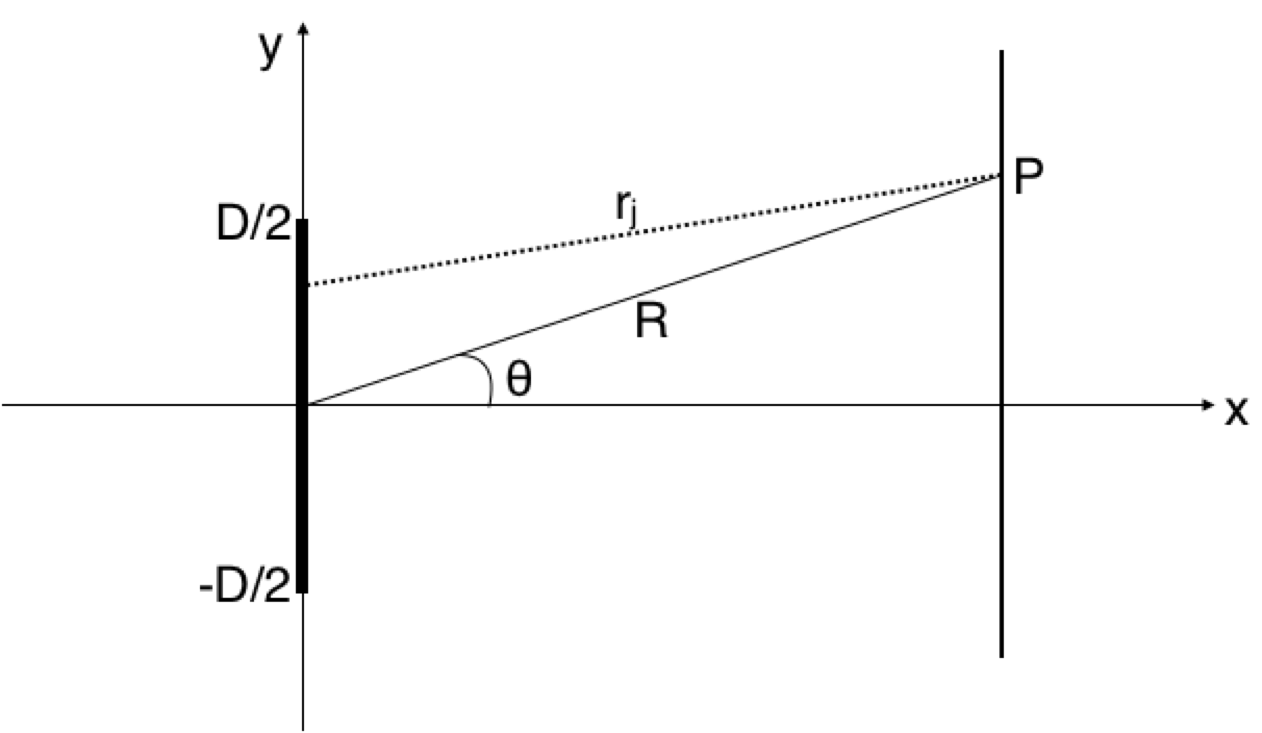
\includegraphics[width=6cm, bb = 0 0 600 200]{SummerChallenge_lineray.png}
\caption{線状光源}
\end{center}
\end{figure}

\clearpage
このとき$\delta y_i$がPに作る電場は、
\[
E_i = \frac{C_0}{r_i} \sin(\omega t- k r_i ) \frac{\delta y_i N}{D}
\]
となる。ただし、$\delta y_i$は微小であり、この微小範囲内の各光源からPまで距離は一定であるとする。さらに一定値の$C_L$を
\[
C_L = \frac{1}{D}  \lim_{N \to \infty} (C_0 N)
\]
と定義できる。M個の全部分によるPでの電場は、
\[
E = \sum_{i=1}^M \frac{C_L}{r_i} \sin(\omega t - k r_i) \delta y_i
\]
最後に、$\delta y_i$は無限小になるはずで、
\[
E = C_L \int_{-D/2}^{D/2} \frac{\sin(\omega t - k r)}{r} dy
\]
となる。ここで、$r = r(y)=\sqrt{R^2 \cos^2 \theta + (R\sin \theta - y )^2}$である。


\subsubsection{単スリット}
まず、単スリットの場合どのように干渉が起こるかを確かめる。振幅、周波数が互いに等しい長さDの線状光源を考える。線状光源の中心からyだけ離れた光源の微小部分dyが、中心からxy平面上の角$\theta$の方向にRだけ離れた点Pに作る電場は、
\[
dE = \epsilon \frac{\sin(\omega t - kr)}{r} dy
\]
$r(y)$を$y$でテイラー展開すると、
\begin{eqnarray*}
r &=&r(0) + \frac{\partial r(0)}{\partial y} y + \frac{1}{2!} \frac{\partial^2 r(0)}{\partial y^2} y^2 + \cdots \\
&=&R - y\sin\theta + \frac{y^2}{2R} \cos^2 \theta
\end{eqnarray*}
となる。いま、$R \gg y$なので、第3項以降は無視できる。
\[
dE = C_0 \frac{sin(\omega t -k(R- ysin\theta ))}{R- ysin\theta} dy
\]
これの分母は$R \gg y$より$R$としてよいので、
\[
dE = C_0 \frac{sin(\omega t -k(R- ysin\theta ))}{R} dy
\]
これは、Rが十分大きいとき、$\theta$の全ての値に対して正しい。
\begin{eqnarray*}
E &=& C_L \int_{-D/2}^{D/2} \frac{\sin(\omega t - k( R - y\sin\theta ))}{R} dy \\
%&=& \frac{C_L}{R} \int_{-D/2}^{D/2} sin(\omega t - k( R - ysin\theta )) \\
&=& \frac{C_L}{R(kD/2)\sin\theta} \sin(\frac{kD}{2} sin\theta) sin(\omega t -kR) \\
&=& \frac{C_L D}{R\beta} sin\beta \sin(\omega t - kR)
\end{eqnarray*}
$\beta = \frac{kD}{2} \sin\theta$とすると、以上のようになり、線状光源が作る電場が導かれた。このとき、強度は$I(\theta) = <E^2>_T$で求められるので、
\begin{eqnarray*}
I(\theta) &=& < E^2>_T\\
&=& <sin^2(\omega t - kR)>_T (\frac{C_L D}{E})^2 (\frac{sin\beta}{\beta})^2
\end{eqnarray*}
$<E^2>_T$は$E^2$の十分に長い時間発展で、周期 $2\pi / \omega$とすると、
\begin{eqnarray*}
 <sin^2(\omega t - kR)>_T  &=& \frac{\omega}{2\pi} \int_{0}^{2\pi / \omega} \sin^2(\omega t - kR) dt \\
 %&=& \frac{\omega}{2\pi} \int_{0}^{2\pi / \omega} \frac{1}{2} (1-cos(2(\omega t -kR))) dt \\
 &=& \frac{1}{2} 
 \end{eqnarray*}
 より、
\[
I(\theta) = \frac{1}{2} (\frac{C_L D}{R})^2 (\frac{sin \beta}{\beta})^2
\]
$I(0)$を求めると
\[
I(0) = \frac{1}{2} (\frac{C_L D}{R})^2
\]
なので、
\[
I(\theta) = I(\theta) (\frac{\sin \beta}{\beta})^2
\]
と求まる。光の強度の変化と観測位置の関係は以下のように表される。\\

\begin{figure}[h]
\begin{center}
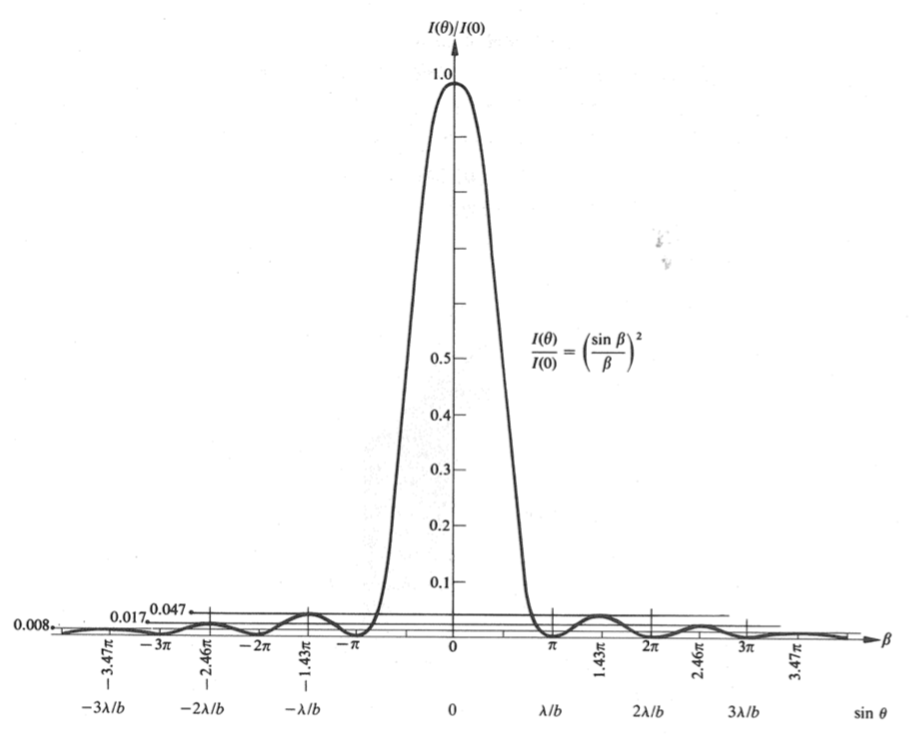
\includegraphics[width=10cm, bb = 0 0 1000 800]{SummerChallenge_slit.png}
\caption{単スリットでの光の強度と角度の関係}
\end{center}
\end{figure}

\clearpage

\subsubsection{2重スリット}
図のような、幅$b$、中心間隔$a$の2本の長いスリットがあるとする。スクリーン上のある点の光波に対する式を得るには、2つの電場の和になるので、
\begin{eqnarray*}
E &=& \frac{C_L}{R} \int_{-b/2}^{b/2} F(z) dz + \frac{C_L}{R'} \int_{a-b/2}^{a+b/2} F(z) dz \\
&\simeq& \frac{C_L}{R} \int_{-b/2}^{b/2} F(z) dz + \frac{C_L}{R} \int_{a-b/2}^{a+b/2} F(z) dz \\ 
\end{eqnarray*}
ここで、
\begin{eqnarray*}
F(z) &=& sin(\omega t - k(R-zsin\theta)) \\
\alpha &=& \frac{ka}{2} \sin\theta \\
\beta &=& \frac{kb}{2} \sin\theta
\end{eqnarray*}
これより、この式を簡単にすると、
\[
E = 2 \frac{C_L b}{R} \frac{\sin\beta}{\beta} \cos\alpha \sin(\omega t -kR + \alpha)
\]
であり、単スリットの時と同様に強度$I(\theta) = <E^2>_T$を求めると、$I(\theta) = \frac{1}{2} (\frac{C_L b}{R})^2$より
\[
I(\theta) = 4I_0 (\frac{\sin \beta}{\beta})^2 \cos^2 \alpha
\]
となる。\\
\\
\\
\\
\begin{figure}[h]
\begin{center}
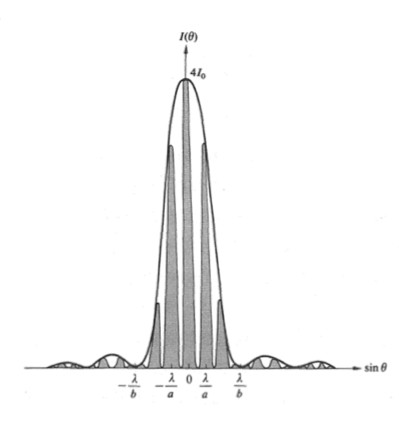
\includegraphics[width=8cm, bb = 0 0 400 300]{SummerChallenge_2slits.png}
\caption{2重スリットでの光の強度と角度の関係}
\end{center}
\end{figure}

\subsubsection{参考文献}
\begin{itemize}
\item 「フーリエ光学(第3版)」森北博巳(森北出版株式会社)2012年初版
\end{itemize}
\clearpage


\subsection{光子を数える}
光量が極端に少なくなると、光は光子として離散的になり、その数を数えることができるようになる。「光子数を数える」ということで、光の粒子性を観測することができる。どのような機器で測定するかは、次章にて述べる。


\section{実験装置}
用いる実験装置は、光検出デバイスMPPC、MPPC読み出しモジュールEASIROC、暗箱、光学機器、スリット、しぼり、LEDです。光学機器を図のように並べ、光の干渉を起こします。各デバイスの位置や距離によって干渉の見え方が変わりますが、これは実際に物を置いていろいろ試してみましょう。以下では、光検出器とその読み出しについて説明します。
\begin{figure}[h]
\begin{center}
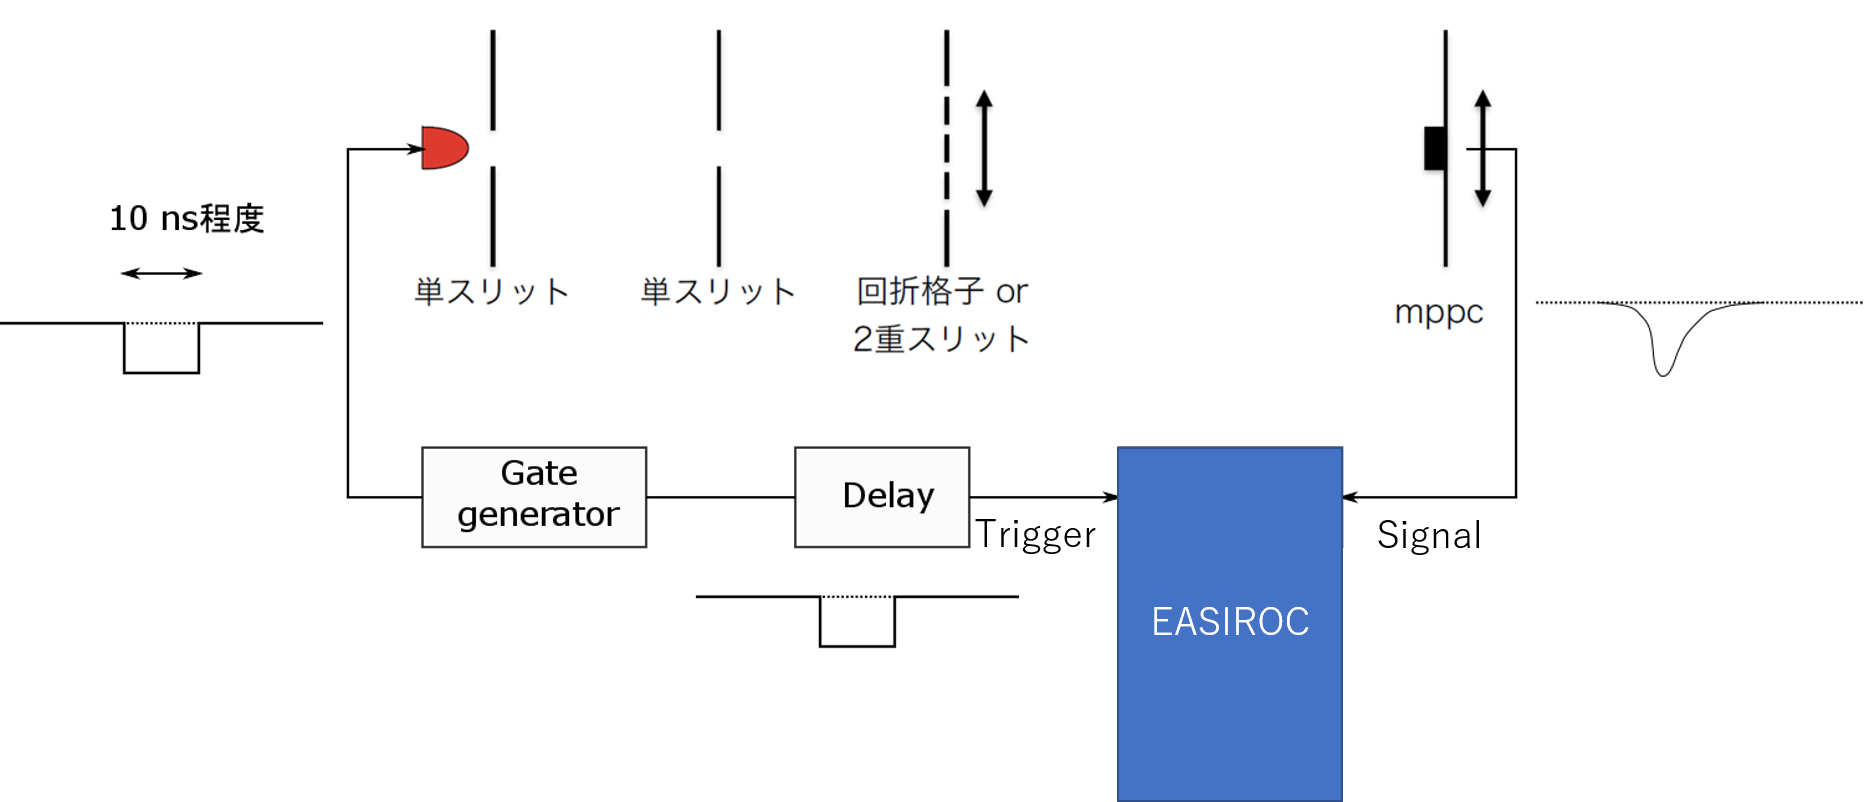
\includegraphics[width=12cm]{setup.PDF}
\end{center}
\caption{セットアップ}
\end{figure}
\subsection{MPPC}
MPPC(Micro Pixel Photon Counter)はAvalamche Photo Diode(APD)が多数配列された光検出器である。APDは半導体でできている。P型とN型、異なるドープ型の半導体にある向きで電圧をかけると、キャリアの少ない空乏層ができる。ここに光子が入射すると、光電効果で電子をはじき出す。電子は印加電圧によってエネルギーを持ち、さらに周囲の原子殻内電子をはじき出し、雪崩(Avalanche)的に電子を倍増する。印加電圧によって様々な倍増モードがあるが、MPPC内のAPDでは、十分な印加電圧をかけることで入射光子数によらない出力電流を得る(ガイガーモード)。このガイガーモードAPDが多数配列することにより、我々は光子が入射したAPDのチャンネル数だけを数えることで、(pile upはあるものの)光子数をデジタルに数えることができる。
\begin{figure}[h]
\begin{minipage}[t]{0.33\hsize}
\begin{center}
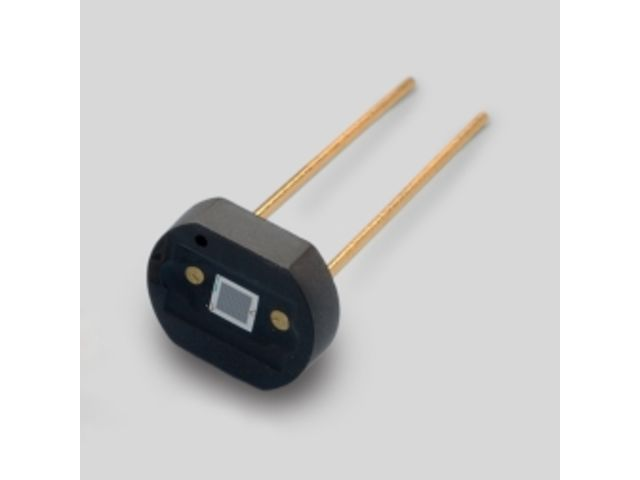
\includegraphics[width=4cm]{mppc.jpg}
\end{center}
\caption{MPPC}
\end{minipage}
\begin{minipage}[t]{0.33\hsize}
\begin{center}
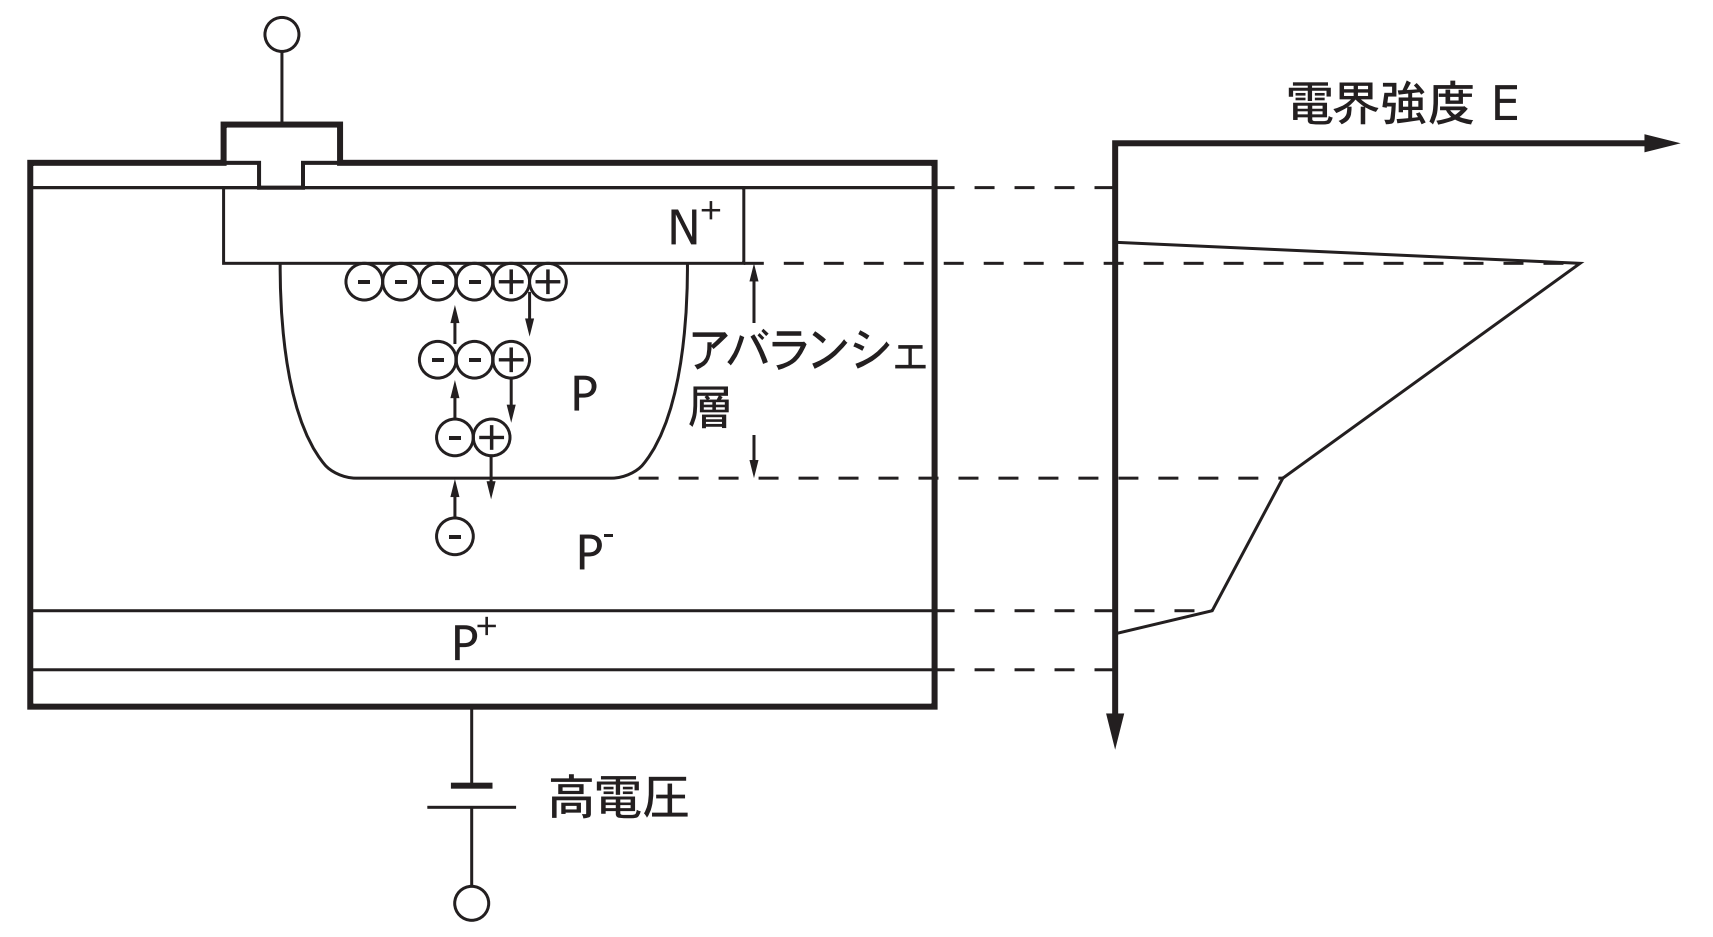
\includegraphics[width=4cm]{APDstructure.PNG}
\end{center}
\caption{APD}
\end{minipage}
\begin{minipage}[t]{0.33\hsize}
\begin{center}
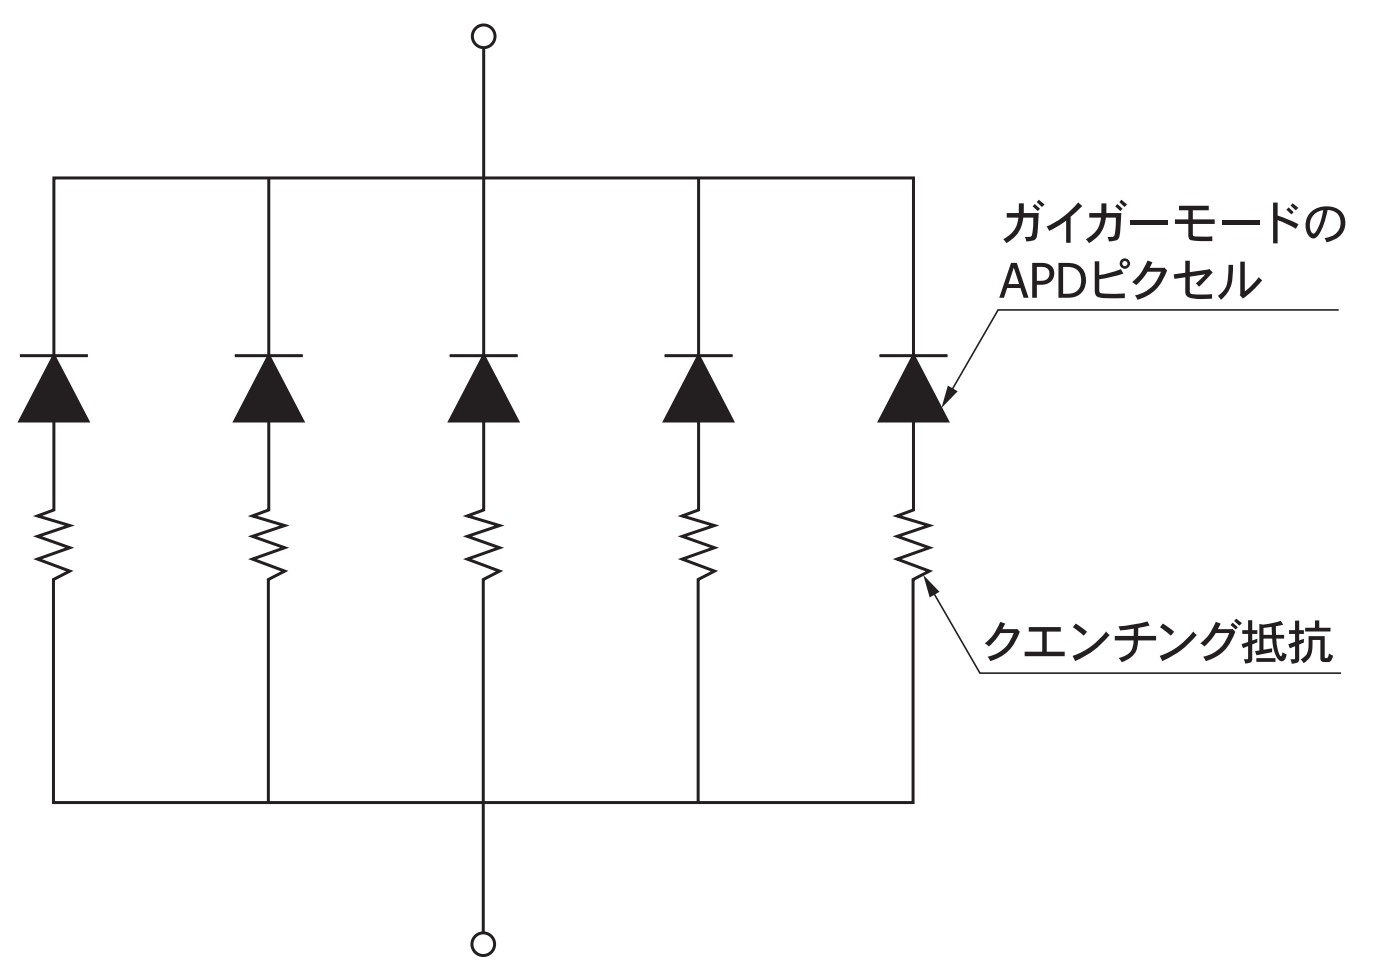
\includegraphics[width=4cm]{QuenchingArray.PNG}
\end{center}
\caption{MPPCはAPDを並列に並べたもの}
\end{minipage}
\end{figure}
浜松ホトニクスのハンドブックに、詳細なMPPCの挙動が説明されている。\cite{hamamatsu}
\subsection{EASIROC}
EASIROCモジュールは、書き換え不可能な集積回路(ASIC)であるEASIROCチップと、EASIROCチップ制御用の書き換え可能な集積回路(FPGA)であるArtix7が搭載された、MPPCの(多チャンネネル)読み出しモジュールである。今回は1チャンネルしか使わないし、FPGAのfirmwareの書き換えも(おそらく)ないので、ここでは、EASIROCチップの回路の概要と、アナログな出力波形について見ることにする。\\
EASIROCチップは、Pre-Amp,Shaper,Discriminator,Capacitorからなる。Pre-Amp,Slow Shaperを通った信号電圧をCapacitorに保存し、Trigger信号が入力されたときに電圧をholdし、ADC(Analog Digital Converter)でデジタル情報に変換する。
\begin{figure}[h]
\begin{center}
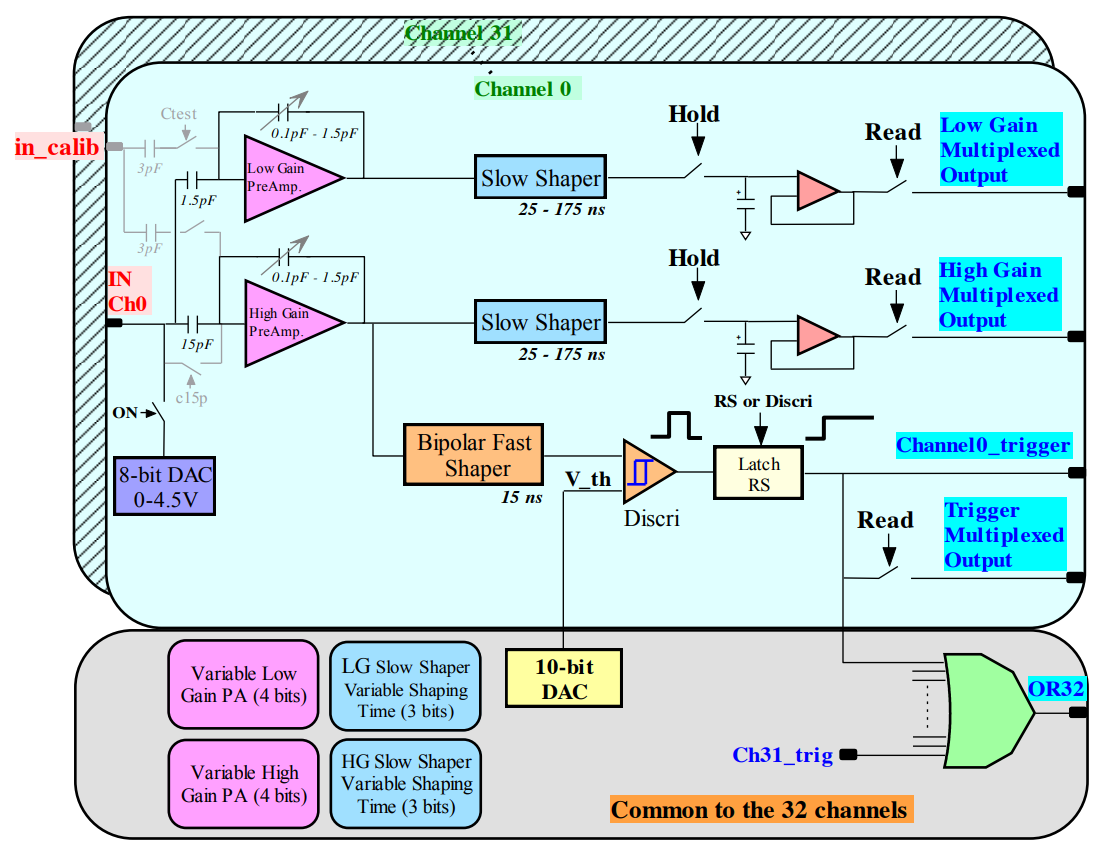
\includegraphics[width=12cm]{EASIROCCircuitDiagram.PNG}
\end{center}
\caption{EASIROC回路概略}
\end{figure}
各デバイスを通った信号の出力波形は、EASIROCモジュールのProbe出力を観察するとわかる。Fast ShaperはSelf Trigger用なので、今回は(おそらく)使わない。Trigger信号に合わせてShaperの波高の一番高いところが読み出されているのがわかる。Trigger信号とShaperの立ち上がりがきちんと合うかどうかはケーブルの長さやDelayモジュールによって操作できる。
\begin{figure}[h]
\begin{minipage}[t]{0.25\hsize}
\begin{center}
\includegraphics[width=3cm]{preamp.BMP}
\end{center}
\caption{Pre-Amp}
\end{minipage}
\begin{minipage}[t]{0.25\hsize}
\begin{center}
\includegraphics[width=3cm]{fastshaper.BMP}
\end{center}
\caption{Fast Shaper}
\end{minipage}
\begin{minipage}[t]{0.25\hsize}
\begin{center}
\includegraphics[width=3cm]{slowshaper.BMP}
\end{center}
\caption{Slow Shaper}
\end{minipage}
\begin{minipage}[t]{0.25\hsize}
\begin{center}
\includegraphics[width=3cm]{slowshaperhold.BMP}
\end{center}
\caption{holdしたSlow Shaper}
\end{minipage}
\end{figure}
\subsection{データ収集の方法}
マニュアル参照

\section{データ解析}
\subsection{MPPCで取得されるデータの解析}
MPPCで取得されるデータはEASIROCによってtree形式で保存される。今回はこのデータをROOTを用いて解析を行う。ここから解析に必要なROOTの知識を簡単に説明するが、すべてを説明することはできないためわからない部分は各自調べるかTAに質問したりするようにしてください。

\subsubsection{ROOTとは}
ROOTとはCERNが開発したデータ解析のためのフレームワークであり、特によく使われる目的としてはヒストグラム・グラフを描く、任意の関数でフィットする、大量のデータを処理するといったものがある。物理学実験では大量のデータを扱うため、例えばエクセルのようなものではそれらのデータをプロットしたり複雑な解析を行うことは難しくなる。そのため、プログラミングによる解析を行えるようになる必要がある。言語としては主にC++で動作し、pythonで書くこともできるが自分がよく知らないため説明はC++のみとなる。また、ROOTで行えることは膨大であるため、できる限り今回必要となる最低限について説明するつもりだがわからない部分も出てくると思うので、それに関してはTAに聞いたり調べたりしてみてください。
ROOTをインストールもしくはROOTがインストールされているマシンにSSH接続して、ROOTを使用できる環境が構築できていることを仮定して、以下で使い方について説明する。

\subsubsection{ROOTの起動方法}
ROOTを起動するためには単にコマンドラインでrootと入力するだけでよい。しかし、rootと入力するだけでは毎回図\ref{fig:ROOT_logo}が表示され、邪魔になるので普段は表示しないようにしたほうがよい。
\begin{figure}[h]
\begin{center}

\includegraphics[width=8cm]{ROOT_logo.png}
\caption{ROOTのロゴ}
\label{fig:ROOT_logo}
\end{center}
\end{figure}
表示させないためには起動させる際にオプションで-lをつければよい。
\begin{table}[hbtp]
  \caption{ROOT起動時のオプションの例}
  \centering
  \begin{tabular}{lcr}
    \hline
    オプション  & 意味 \\
    \hline \hline
      -l:  & 起動時にロゴを表示しない  \\
      -b:  & ヒストグラムやグラフのグラフィックを描画しない \\
      -q:  & スクリプトファイルを実行後自動でROOTが終了する \\
    \hline
  \end{tabular}
\end{table}
ROOTを終了したいときには、.qと入力すればROOTを終了させることができる。

\subsubsection{ヒストグラムの描き方}
rootを起動する際に、引数にrootファイルを指定することでrootの起動と同時にROOTファイルを開くことができる。例えば、今回測定結果をexample.rootという名前で保存しているとした場合、root example.rootとコマンドラインから入力することで測定データに簡単にアクセスすることができる。\ref{fig:open_ROOT}
\begin{figure}[h]
\begin{center}
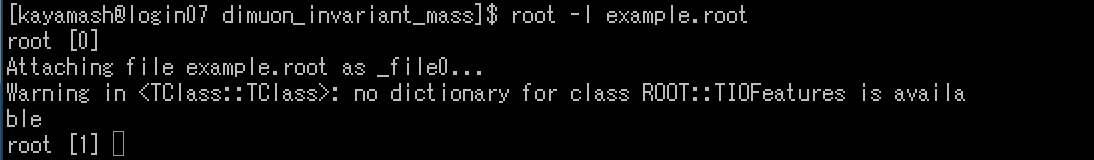
\includegraphics[width=8cm]{SummerChallenge_open_root.png}
\caption{rootファイルを開く}
\label{fig:open_ROOT}
\end{center}
\end{figure}

example.root内にさらにtreeという名前でtreeを作っている場合、tree-$>$''コマンド''という書き方をすることができる。それにより、簡単に測定データを確認したりヒストグラムを描くことができる。コマンドとしては例えば、tree-$>$Print$\left(\right)$やtree-$>$Scan$\left(\right)$があり、Printはデータの数や種類、変数の方を確認でき、Scanは1つ1つのデータを実際に確認することができる。
\begin{figure}[htbp]
\begin{center}
  \begin{tabular}{c}

    \begin{minipage}{0.5\hsize}
      \begin{center}
        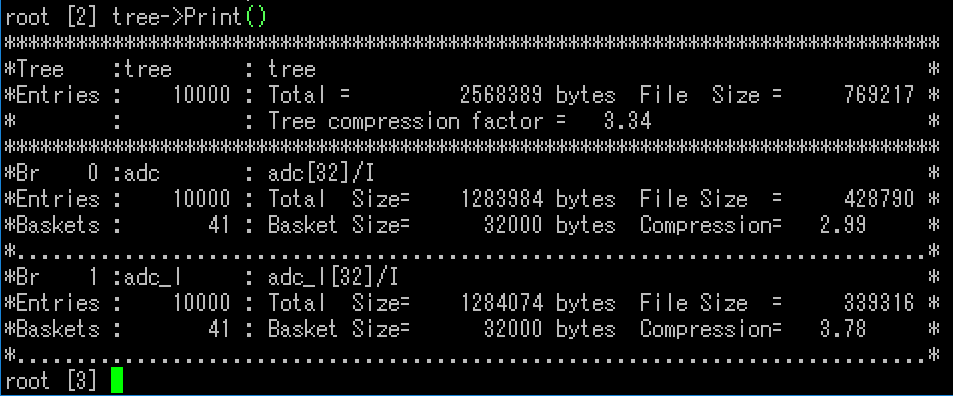
\includegraphics[clip, width=60mm]{SummerChallenge_tree_print.png}
        \hspace{1.6cm} (a)tree-$>$Print$\left(\right)$の実行例
      \end{center}
    \end{minipage}

    \begin{minipage}{0.5\hsize}
      \begin{center}
        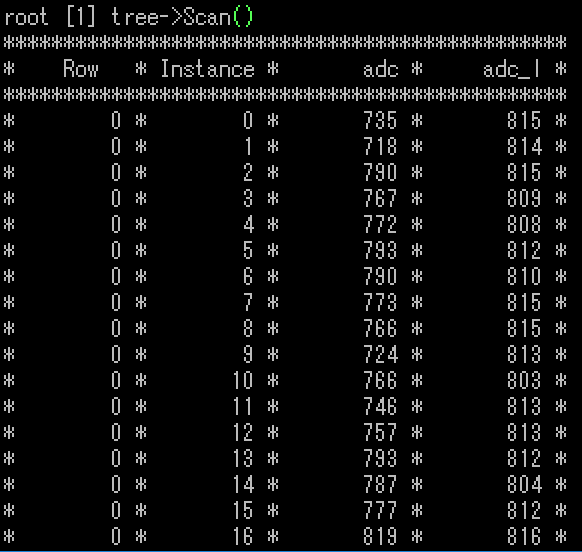
\includegraphics[clip, width=60mm]{SummerChallenge_tree_scan.png}
        \hspace{1.6cm} (b)tree-$>$Scan$\left(\right)$の実行例
      \end{center}
    \end{minipage}
  \end{tabular}
  \end{center}
\end{figure}

今回treeの中身をPrintやScanで確認すると、いくつかのBranchがあると思う。\footnote{Branchとは言葉通り枝のようなもので、1つのEntryに対して様々なデータを詰め込むことができる。}そのうち今回adcというBranchのヒストグラムを描きたい場合、tree-$>$Draw$\left(''adc''\right)$と打つだけでヒストグラムを描くことができる。\footnote{今回、EASIROCでは32chのデータが配列としてadcのBranchに入っており、そのうちMPPCがつながっているのは30chのみなので、adc[30]のみをDrawすることで測定データのヒストグラムを描ける}
\begin{figure}[htbp]
\begin{center}
  \begin{tabular}{c}

    \begin{minipage}{0.5\hsize}
      \begin{center}
        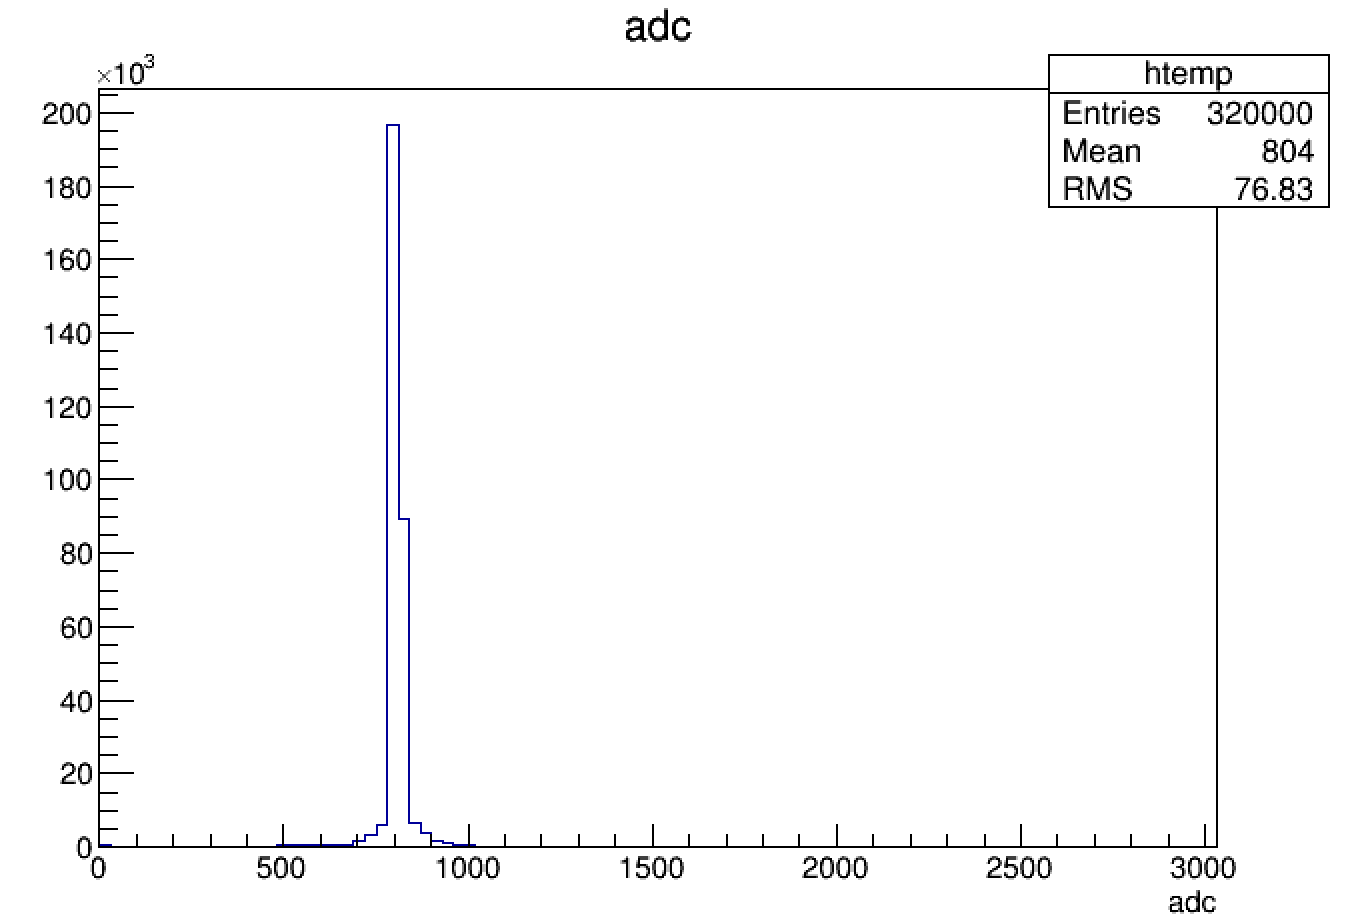
\includegraphics[clip, width=60mm]{SummerChallenge_tree_draw_adc.png}
        \hspace{1.6cm} (a)tree-$>$Draw(''adc'')の実行例
      \end{center}
    \end{minipage}

    \begin{minipage}{0.5\hsize}
      \begin{center}
        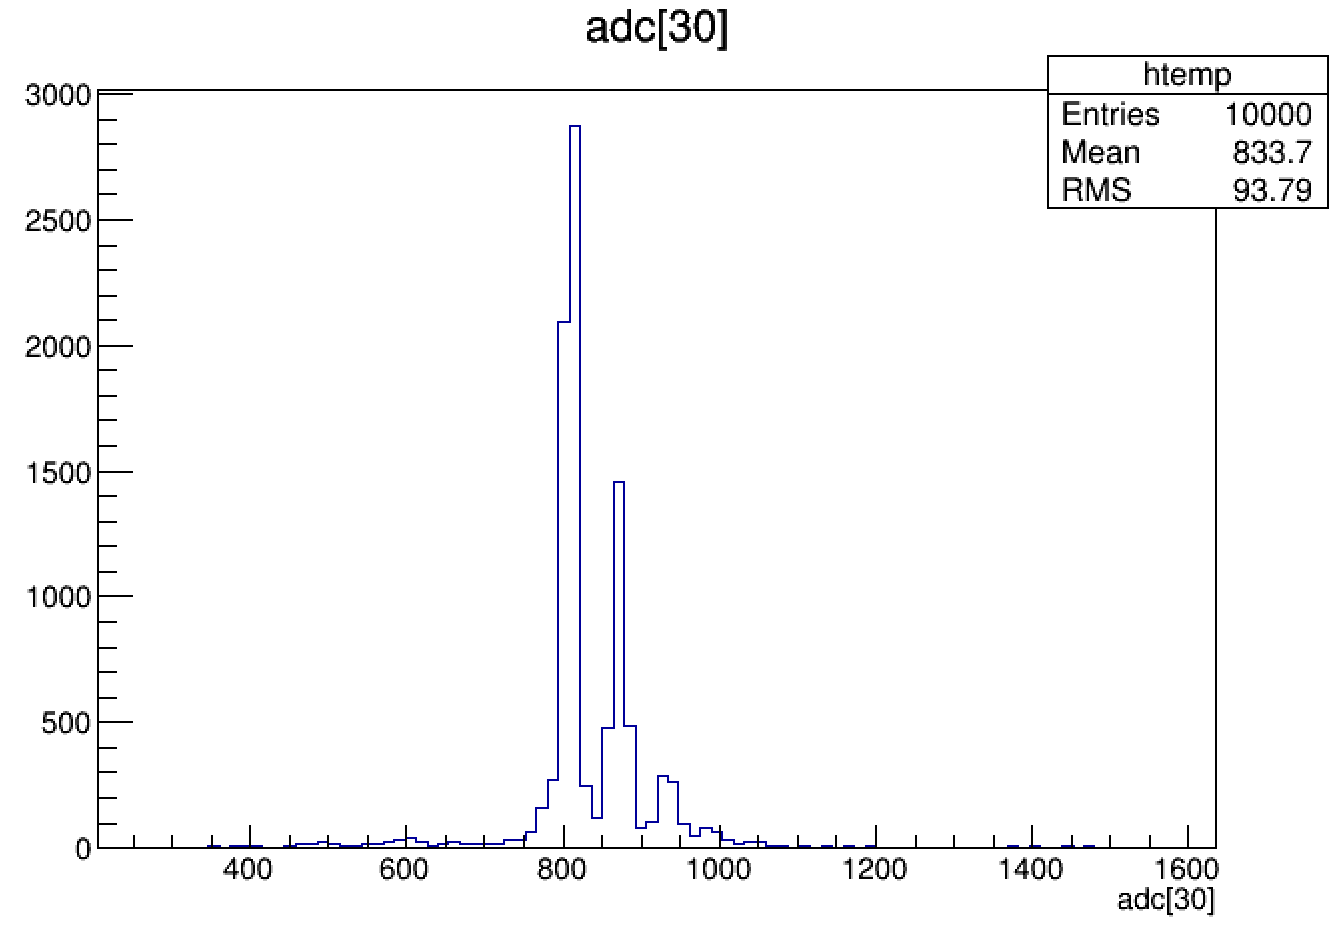
\includegraphics[clip, width=60mm]{SummerChallenge_tree_draw_adc30.png}
        \hspace{1.6cm} (b)tree-$>$Draw(''adc[30]'')の実行例
      \end{center}
    \end{minipage}
  \end{tabular}
  \label{fig:tree_draw}
  \end{center}
\end{figure}

ヒストグラムを書くときに、ただそのまま書くだけでなく様々な条件をかけることもできる。例えば、tree-$>$Draw(''adc*2'')とすれば、adcの値を2倍したヒストグラムを描くことができ、tree-$>$Draw(''adc'',''adc>900'')とすればadcが900より大きいイベントのみ描くことができます。この条件には、ほかのBranchを用いることもできtree-$>$Draw(''adc'',''adc\_l $>$ 1000 \&adc\_l $<$ 3000'')とすれば1000$<$adc\_l$<$3000のみのヒストグラムを描くことができる。ただし、ある程度複雑な条件になってくるとこの書き方をするのは難しくなってくるので、後述するマクロを書いてヒストグラムを描くことをお勧めする。

最後にtreeをそのままdrawする以外のヒストグラムの描き方として、Fillという方法がある。簡単な例として、自分でガウス分布に従う乱数を発生させてそれをヒストグラムに詰めるやり方を紹介する。
\begin{lstlisting}[basicstyle=\ttfamily\footnotesize, frame=single]
    TH1D *h1 = new TH1D(''h1'',''h1'',50,-5,5);
    for(Int_t i = 0;i < 10000;i++){
     Double_t x = gRandom->Gaus();
     h1->Fill(x);
    }  
    h1->Draw();
 \end{lstlisting}
 3行目でgRandomというものを用いてGauss分布に従う乱数を発生させ、それを4行目でFillというコマンドでh1のヒストグラムに詰めている。それをfor文で回して10000回詰めている。このヒストグラムをDrawすることでGauss分布に従うヒストグラムを描くことができる。今回は例として乱数をFillしたが、乱数の代わりに詰めたい値を詰めることで好きなヒストグラムを描くことができる。

\subsubsection{マクロの書き方}
簡単なマクロはコマンドラインに書いてヒストグラムを描くときと同じものを描くだけでよい。ただし、rootファイルを読み込む際には必要な手順があるので例としてそれを示す。
\begin{lstlisting}[basicstyle=\ttfamily\footnotesize, frame=single]
void macro(){
	TFile *file = new TFile("example.root");
	TH1D *h1 = (TH1D*)file->Get("adc");
	h1->Draw();
}
 \end{lstlisting}
というファイルを作り、ターミナル上でroot macro.cxxやrootを起動した後、.x macro.cxxとコマンドすることでこのマクロを実行できる。
データの解析には基本的にはROOT固有の知識はそれほど必要ではなく、c++の知識があれば充分であるため深くは説明しない。

もう一つ必要な知識として、詳しい解析を行う際にはBranchのデータをヒストグラムとしてではなく値として取り出す必要がある。そのためこれも簡単にではあるが、値としての取り出し方を説明する。

\begin{lstlisting}[basicstyle=\ttfamily\footnotesize, frame=single]
void macro(){
    TFile *file = new TFile(inputfilename, "read"); 
    TTree *tree = (TTree*)file->Get("tree");
 
    Double_t adc[32]
    tree->SetBranchAddress("adc", &adc);
 
    const Int_t N = tin->GetEntries();
    for (Int_t ientry = 0; ientry < N; ientry++) {
     tree->GetEntry(ientry);    
     cout<<ientry<<''   ''<<adc[30]<<endl;
   }
}
 \end{lstlisting}

tree-$>$GetEntry(ientry)とすることで、ientry番目のイベントのadcを読み込んでおり、それをfor文で全イベント回すことで全データを読み込んでいる。今回のマクロではcoutで出力しているだけだが、その値をvectorや配列に詰めることで解析に用いることができる。

コマンドラインによる解析の仕方も一応説明しているが、測定直後にデータを簡単に確認したいといった場合を除いてはマクロを用いればよい。また、データを確認する場合でもTBrowser\footnote{ROOTを起動した後、TBrowser tbと入力することでrootファイルの中身をヒストグラムとして簡単に見ることができる}が便利であるため、あまり使用頻度は高くないと思われる。

\subsubsection{ヒストグラムのフィット}
ROOTにはあらかじめガウス分布やポアソン分布などの様々な関数が用意されており、それらをヒストグラムのフィットを行う際に利用できる。例えばガウス分布でフィットする際には、htemp-$>$Fit(''gaus'')とすればよい。\footnote{htempの部分はその時のヒストグラムの名前に応じて適宜変える}コマンドラインで行った場合にはコマンドラインにfitの結果が出力される。
\begin{figure}[h]
\begin{center}
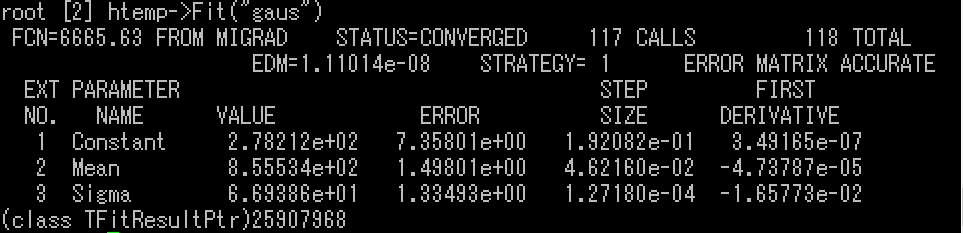
\includegraphics[width=8cm]{SummerChallenge_fit_gaus.png}
\caption{フィットの結果}
\label{fig:fit_gaus}
\end{center}
\end{figure}

ガウス分布の場合は、$(gaus)=(Constant)\times$exp$(-\frac{(x-(Mean))^2}{2(Sigma)^2})$で定義されている。それぞれの出力されるパラメータは関数によって異なるため、ほかの関数を用いる際は一度確認しておくとよい。
また、htemp-$>$Fit(''gaus'','''','''',min,max)とすることでフィットする範囲を制限することができる。

あらかじめ定義されている関数以外の関数を用いたい場合は自分で定義することができる。例えば直線でフィットしたい場合には、
\begin{lstlisting}[basicstyle=\ttfamily\footnotesize, frame=single]
TF1 *f1 = new TF1(''f1'',''[0] + [1] * x'',min,max);
 \end{lstlisting}
とすることでまず直線の関数を定義することができる。この関数の名前はf1になっているので、あとは先ほどガウス分布でフィットしたときと同様に、
\begin{lstlisting}[basicstyle=\ttfamily\footnotesize, frame=single]
htemp->Fit(''f1'','''','''',min,max);
 \end{lstlisting}
とすればよい。

フィットする際にある程度のパラメータを指定したい場合がある。その際にはf1->SetParameter(0,5)とすれば0番目のパラメータの初期値を5に設定でき、f1->SetParameters(5,10)とすればまとめて複数のパラメータの初期値を設定できる。

マクロで行う場合には基本的には同じだが、フィットした結果をマクロ内で用いたい場合は値として取り出す必要がある。
\begin{lstlisting}[basicstyle=\ttfamily\footnotesize, frame=single]
Double_t p0 = f1->GetParameter(0);
 \end{lstlisting}
とすると、p0にフィットした後の0番目のパラメータの値を代入することができる。

\subsubsection{グラフの描き方}
基本的な使い方として、テキストファイルからグラフを描くやり方と配列やvector\footnote{vectorが何かわからない場合はc++の勉強が先に必要なため、c++ vector等で検索して使い方を勉強したほうがよいでしょう}を用いる方法がある。まずはテキストファイルでのグラフの書き方から説明する。

例としてdata.datというファイルに
\begin{lstlisting}[basicstyle=\ttfamily\footnotesize, frame=single]
1.00 3936
0.50 3007
0.10 2249
-0.10 1836
-0.50 1097
-1.00 146
 \end{lstlisting}
 と書かれている場合、簡単にグラフを描くことができ
\begin{lstlisting}[basicstyle=\ttfamily\footnotesize, frame=single]
TGraph *tg1 = new TGraph(''data.dat'');
tg1->Draw(''AP'');
 \end{lstlisting}
とするだけでグラフを描くことができる。ただし、この方法を用いるためには結果をまずdatファイルとして出力する必要があるため、あまり使うことはないだろう。

配列やvectorを用いる場合、まずは配列やvectorにデータを詰める必要があり、その部分は省略する。すでに値が詰まっていると仮定すると、配列の場合は
\begin{lstlisting}[basicstyle=\ttfamily\footnotesize, frame=single]
TGraph *tg1 = new TGraph(6,x,y);
tg1->Draw(''AP'');
 \end{lstlisting}
とすると、6個のデータを含むグラフを描くことができる。しかし、測定データによってグラフが何点あるかは異なる場合もあり、vectorを用いたほうが様々な場合に柔軟に用いることができ便利である。

vectorを用いた場合は
\begin{lstlisting}[basicstyle=\ttfamily\footnotesize, frame=single]
TGraph *tg1 = new TGraph(x.size(),&(x.at(0)),&(y.at(0)));
tg1->Draw(''AP'');
 \end{lstlisting}
c++の知識がある人は、これを見てやってることは同じだとわかると思う。

また、グラフにエラーバーをつけたい場合も多いと思う。その場合はTGraphではなくTGraphErrorsを用いればよい。使い方はほとんど同じで、
\begin{lstlisting}[basicstyle=\ttfamily\footnotesize, frame=single]
TGraph *tg1 = new TGraph(6,x,x_error,y,y_error);
tg1->Draw(''AP'');
 \end{lstlisting}
 の順番に引数がなっており、その通りにTGraphの時と同様に配列やvectorで与えればよい。

最後にグラフのフィットについてであるが、ヒストグラムの場合と全く同じであり例えば直線でフィットしたい場合には
\begin{lstlisting}[basicstyle=\ttfamily\footnotesize, frame=single]
TF1 *f1 = new TF1(''f1'',''[0] + [1] * x'',min,max);
tg1->Fit(''f1'','''','''',min,max);
 \end{lstlisting}
とすればグラフを直線でフィットすることができる。

\subsubsection{結果の保存}
コマンドラインで結果のヒストグラムやグラフを保存する場合には、左上のFileからSave Asを選ぶと名前を付けて保存することができる。マクロで実行している場合には、ヒストグラムやグラフを描く前に
\begin{lstlisting}[basicstyle=\ttfamily\footnotesize, frame=single]
TCanvas *c1 = new TCanvas(''c1'',''c1'',1600,900);
 \end{lstlisting}
としてキャンバスを作っておき、ヒストグラムやグラフをDrawした後に
\begin{lstlisting}[basicstyle=\ttfamily\footnotesize, frame=single]
c1->SaveAs(''save name'');
 \end{lstlisting}
とすることで保存することができる。保存する際にきれいにヒストグラムやグラフを整えた後、保存したい人も多いと思う。rootはヒストグラムやグラフそれぞれに様々な修飾等が存在し、それをここで説明しているときりがないためまとめ\ref{sec:lastsection}にそれらが書かれているリンクを載せておく。

また、ヒストグラムを保存する際に画像としてでなくrootファイルにヒストグラムのまま保存することができる。実際に触ってみないとそのメリットは感じにくいかもしれないが、rootファイルの状態で保存することで、保存した後にタイトルをつけたりbin幅を変えるといった加工が簡単に行える。そのため、最終的にスライド等に用いる時以外はrootファイルで保存しておいたほうが便利かもしれない。具体的なやり方が書かれているサイトのリンクをここに載せておく。\footnote{\url{https://www-he.scphys.kyoto-u.ac.jp/member/n.kamo/wiki/doku.php?id=study:software:root:io}のWrite ・オブジェクトをファイルに書き込む、rootファイルを保存するを参考にしてもらえばよい。}なお、ヒストグラム等を保存する際は測定データのrootファイルとは別に保存用のrootファイルを作るようにしてください。測定データを上書きしてしまうリスクを避けるために、測定データは読み込み専用で開く習慣をつけるためである。

\subsection{Poisson統計}
Poisson分布とはめったに起こらない事象を大量に測定した場合にこの分布に従うことが多い。式で表すと、
\begin{equation}
P\left(n\right)=\frac{\lambda^n e^{-\lambda}}{n!}
\end{equation}
で、これは平均$\lambda$起こる事象がn回起こるときの確率を表す。今回の実験の場合はそれぞれの測定での光子数の分布はPoisson分布に従うと思われる。
\begin{figure}[h]
\begin{center}
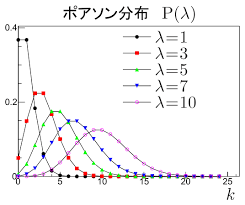
\includegraphics[width=8cm]{SummerChallenge_poisson.png}
\caption{poisson分布の図}
\label{fig:poisson}
\end{center}
\end{figure}

$\lambda$が大きい場合はPoison分布はGauss分布(正規分布)に従う。今回の実験の場合では、それぞれの光子数に対応するピークはGauss分布に従うと思われる。
\begin{figure}[h]
\begin{center}
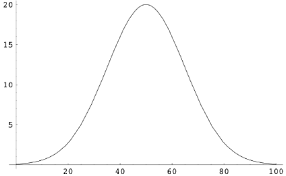
\includegraphics[width=8cm]{SummerChallenge_gauss.png}
\caption{gauss分布の図}
\label{fig:gauss}
\end{center}
\end{figure}

\subsection{干渉縞の再現}
今回の測定データは最初adcの値として保存されており、この値自体に物理的な意味はない。そのため、まずはこの値から光子数に変換する必要がある。やり方としてはそれぞれのピークが光子数に対応しているため、それぞれをガウス分布でフィットして中心値を求める。そのadc値と光子数の関係を直線近似することで横軸をadcから光子数に変換することができる。

そのあと、変換した後のヒストグラムからMPPCの位置ごとの平均光子数を求めてプロットすることで干渉縞を再現することができる。平均光子数については様々な求め方があるが、簡単なものについては光子数で重みづけした平均、もう少しちゃんと求める場合には上で述べたように光子数の分布はPoisson分布に従うため、全体をPoisson分布でフィットすることで求めるほうがよい。

また、演習3で光子数を減らした場合はフィットで平均光子数を求めることは難しい。その場合は平均光子数ではなく1光子以上のイベント数で考えるとよい。平均光子数そのものではないが、光子数が少ない場合には平均光子数に比例して1光子以上のイベント数も増加するため、それでも干渉縞を観測することができる。\footnote{物理的な説明をすると、1光子の干渉と仮定すると明線の部分では光子の存在確率が大きいため、光子を観測するイベント数が増加する。光子数が増加すると光子数0となるイベントは暗線であっても減少するため、この考え方で解析することは難しくなる。}

\section{まとめ}
\label{sec:lastsection}
今回説明できたのはごく基本的な部分のみであり、今回の実験の解析についてもこれ以上の知識が必要になることがあると思う。c++の知識でわからないことがあれば

\url{http://www7b.biglobe.ne.jp/~robe/cpphtml/}
の第1部を見ればある程度の情報はのっていると思われる。もし、これにのっていない知識が必要になれば別途調べるか質問してください。

ROOTについての情報は基本的なものは

\url{http://www-ppl.s.chiba-u.jp/~hiroshi/ref/ROOT_text.pdf}

\url{https://www.quark.kj.yamagata-u.ac.jp/~miyachi/ROOT/root.pdf}

、途中で話した修飾については

\url{http://atlas.kek.jp/comp/ROOT-commands.html} 

を見ればある程度一覧になっている。もし、そこにのっていない知識が必要になったときは別途調べるか、

\url{https://root.cern.ch/guides/users-guide}

のUser's Guideを見ればわかると思うが、User's Guideは英語の上膨大であるため、適宜調べるのがよいと思う。

また、あまり全てを書きすぎると参加している皆さんが考えることがなくなってしまうため、あえて説明をしていない部分もある。なので、この資料を読んでわからないことがあれば遠慮せずにどんどん聞いてください。

\end{document}
\begin{thebibliography}{9}
\bibitem{hamamatsu}
https://www.hamamatsu.com/resources/pdf/ssd/03\_handbook.pdf
\end{thebibliography}
